\documentclass[12pt]{article}
\usepackage[utf8]{inputenc}
\usepackage[a4paper,margin=0.8in]{geometry}
\usepackage{amsmath}
\usepackage{amssymb}
\usepackage{graphicx}
\usepackage{float}
\usepackage{tabularx}
\usepackage{gensymb}
\usepackage{caption}
\usepackage{subcaption}
\usepackage{array}
\usepackage{multirow}
\usepackage{listings}
\usepackage[dvipsnames]{xcolor}
\usepackage{pythonhighlight}
\usepackage{fancyhdr}
\usepackage{mathtools}
\setlength{\parindent}{0em}
\usepackage{pgfplots}
\pgfplotsset{compat=1.18}
\usepackage[framemethod=tikz]{mdframed}
\usepackage[colorlinks=true, breaklinks = true, linkcolor = black, urlcolor=blue]{hyperref}
\usepackage{xurl}
\usepackage{booktabs}
\usepackage{multicol}
\definecolor{keyred}{RGB}{165,25,25}
\newcommand{\key}[1]{\textcolor{keyred}{\textbf{#1}}}
\setlength{\parskip}{0.55em}
\graphicspath{{../img/}{./}}
\renewcommand{\arraystretch}{1.25}
\newcolumntype{L}{>{\raggedright\arraybackslash}X}
\captionsetup{font=small,labelfont=bf}
\renewcommand{\topfraction}{0.9}
\renewcommand{\bottomfraction}{0.8}
\renewcommand{\textfraction}{0.07}
\renewcommand{\floatpagefraction}{0.75}
\setcounter{topnumber}{3}
\setcounter{totalnumber}{4}
\mdfdefinestyle{note}{linecolor=keyred,linewidth=1pt,roundcorner=4pt,backgroundcolor=keyred!4,innertopmargin=8pt,innerbottommargin=8pt}

\title{
\begin{center}
        \huge{\textbf{Indian Institute of Technology Madras}}\\
        \huge{Department of Engineering Design}\\
        \vspace{1em}
        \LARGE{ED5012 : Advanced Applications of Human Factors in Design}\\
        \vspace{1em}
        \LARGE{Term Project : FormDrift}\\
        \vspace{0.4em}
        \Large{Detecting Exercise-Technique Drift That Lifters Cannot Perceive}\\
         \vspace{1em}
    \end{center}

    \begin{figure}[H]
    \vspace{1.5em}
        \centering
        
\includegraphics[width=10cm]{Logo.png}
    \end{figure}
    \vspace{1em}
    \begin{center}
        \LARGE{Vinnay Gupta}\\
        \LARGE{ED22B073}\\
    \end{center}
}
\date{}
\begin{document}
\pagenumbering{gobble}
\maketitle
\newpage
\pagenumbering{arabic}
\pagestyle{fancy}
\renewcommand{\footrulewidth}{0.4pt}
\renewcommand{\sectionmark}[1]{\markboth{#1}{#1}}
\fancyhead{}
\fancyhead[L]{\small ED5012 Term Project}
\fancyhead[R]{\small FormDrift}
\fancyfoot[C]{\thepage}

\section*{Abstract}

People who train without a coach rarely notice their technique deteriorating within a set. They cannot see themselves, joint-position sense becomes less accurate as muscles fatigue, and the change from one repetition to the next is small. This project, \key{FormDrift}, is a Progressive Web App (PWA) that analyses a squat video on the user's own device. It builds a personal baseline from the lifter's first repetitions, measures how each later repetition departs from that baseline (depth, trunk lean, knee tracking, lateral hip shift, concentric velocity and movement shape), gives at most one short cue per repetition, and ends with a summary that explains what changed, why it matters and what to do about it.

The work follows the course's 4W1H framework and the five-level ladder that pairs user characteristics with work characteristics: anthropometry, biomechanics, information handling, functional evaluation and aesthetic evaluation. On simulated fatigue sets with known ground truth, the analyser counted 10 of 10 repetitions from both side and front cameras and flagged drift with a precision and recall of 1.00. The mean absolute error was 0.7\% of leg length for depth and 0.8\degree\ for trunk lean, and the F1 score stayed at or above 0.92 with up to 10 pixels of added landmark noise. On two real, Creative Commons licensed videos it counted 10 of 10 repetitions with no false technique alarms. The app needs only a browser, so every claim in this report can be checked live.

\begin{mdframed}[style=note]
\textbf{Live application:} \url{https://formdrift.apps.grok.bot}\\
\textbf{Source code:} \url{https://github.com/vinnay4/ED5012}\\
\textbf{Slides:} built into the app at \texttt{\#/present} (press F for full screen).
\end{mdframed}

\setcounter{tocdepth}{1}
\begingroup\setlength{\parskip}{0pt}\small
\renewcommand{\contentsname}{}
\section*{Contents}\vspace{-2.2em}
\begin{multicols}{2}
\tableofcontents
\end{multicols}
\endgroup
\newpage

%=====================================================================
\section{Introduction}

\subsection{Course brief}

The ED5012 term project asks for a human factors problem in one of several application domains, analysed with the 4W1H framework (who, when, where, what and how) and the user-versus-work characteristics ladder taught in the course. Two checks must be passed before a problem is accepted: the problem must be a human issue, and the solution must be demonstrable as a Progressive Web App. I chose the \key{Intelligent Sports} domain and, within it, unsupervised resistance training.

\subsection{Why resistance training}

Resistance training has become largely self-directed. Many people follow programmes from videos or apps, train at home or at off-peak hours, and meet a coach rarely or never. The squat is the most common lower-body exercise in these programmes, and its technique faults are well documented in the strength and conditioning literature (Myer et al., 2014; Parmar and Morris, 2022). Commercial motion-analysis products for athletes exist, but most need dedicated sensors or wearables. A phone or laptop camera combined with on-device pose estimation can give similar feedback to anyone who already owns a phone.

%=====================================================================
\section{Problem Statement}

\subsection{The human issue}

\begin{mdframed}[style=note]
\textbf{Lifters training without supervision do not recognise that their technique is deteriorating across the repetitions of a set.}
\end{mdframed}

There are four causes, and all of them lie in human capability rather than in missing technology.

\begin{enumerate}
    \item \textbf{No external view.} The lifter cannot see their own sagittal-plane form. A mirror shows only the frontal plane, and looking at it pulls the head out of a neutral position.
    \item \textbf{Proprioception degrades with fatigue.} Muscle fatigue reduces the accuracy of joint-position sense and force sense (Proske and Gandevia, 2012). This happens in the last repetitions of a set, which is also when technique starts to slip.
    \item \textbf{The change is gradual.} Depth may shrink by a few percent per repetition and the chest may drop by a few degrees. No single repetition feels wrong, so the change stays below the threshold of noticing.
    \item \textbf{Bodies differ.} Generic rules such as ``thighs parallel'' or ``back at 45\degree'' ignore the fact that a lifter with a long femur relative to the trunk must lean further forward than a short-femur lifter to reach the same depth. Self-checks based on generic rules therefore misjudge many people.
\end{enumerate}

The consequences are a reduced training stimulus (shallower repetitions), higher spinal loading (more trunk flexion under load) and more stress on the knee (dynamic valgus). Feedback, when it is given, is often a screen full of numbers that competes for attention during exertion and can make performance worse.

\subsection{The two mandatory checks}

\begin{table}[!htbp]
\centering
\caption{The two checks required by the course brief.}
\begin{tabularx}{\textwidth}{>{\raggedright\arraybackslash}p{3.4cm} >{\raggedright\arraybackslash}p{2.2cm} L}
\toprule
\textbf{Check} & \textbf{Verdict} & \textbf{Reasoning} \\
\midrule
1. Is it a human issue? & Yes & The root causes are limits of human perception, proprioception under fatigue, anthropometric variation, and attention and workload during exertion. Better sensors alone cannot fix this; the feedback has to be designed around the person receiving it. \\
2. Can it be built and presented as a PWA? & Yes, and demonstrated & MediaPipe Pose Landmarker runs in the browser through WebAssembly and WebGL. The analysis is written in TypeScript, audio cues use the Web Speech API and haptic cues use the Vibration API. A service worker makes the app installable and usable offline. There is no server and no extra hardware, and video never leaves the device. \\
\bottomrule
\end{tabularx}
\end{table}

%=====================================================================
\section{Users, Context and Task}

\subsection{User profile}

The target user is a recreational or intermediate lifter, roughly 18 to 35 years old, with at least six months of training experience, so that the loads used are heavy enough for fatigue to matter. Users train alone, from online programmes or with a coach they see only occasionally. They vary widely in stature (about 1.5 to 1.9 m), in segment proportions such as the femur-to-trunk ratio, in ankle and hip mobility, and in sex. A large share of the intended users are Indian, a population whose body dimensions differ from the Western data most guidelines are based on (Chakrabarti, 1997).

\subsection{Usage scenario}

Arjun, 24, trains in a residential gym three evenings a week. He props his phone against a dumbbell rack about two and a half metres away, side-on, and records a set of ten goblet squats. By the eighth repetition his legs are burning; he feels he is squatting as before, but his hips are stopping higher and his chest is dropping. After the set he opens FormDrift, loads the clip and answers one question: ``When did your form start to slip?'' He says rep 8. The app shows that measurable drift began at rep 6, that his depth fell by about a quarter and his trunk lean grew by 18\degree, and it suggests ending the set earlier next time and practising a tempo goblet squat. During later sets, the audio channel gives him a two-word cue at the top of a repetition when something changes, and otherwise stays quiet.

\subsection{Task analysis of a squat set}

\begin{table}[!htbp]
\centering
\caption{Phases of a working set and the human factors demands in each.}
\begin{tabularx}{\textwidth}{>{\raggedright\arraybackslash}p{3.0cm} L L}
\toprule
\textbf{Phase} & \textbf{What the lifter does} & \textbf{Implication for the design} \\
\midrule
Set-up & Places the phone, steps into position, picks up the load & Filming guidance must be simple: hip height, 2--3 m away, side-on for trunk lean or front-on for knee tracking. \\
Early repetitions & Moves with fresh muscles and good control & These repetitions are the most representative of the lifter's own technique, so they form the baseline. \\
Bottom of each repetition & Highest muscular effort and balance demand & No feedback is given here; attention is fully on the lift. \\
Top of each repetition & Brief standing pause & This is the moment for a cue, if one is needed. \\
Late repetitions & Fatigue builds and form drifts & This is where drift detection, a priority order and a possible ``end the set'' message are needed. \\
After the set & Rests for one to three minutes & There is time to read charts, explanations and drills. \\
\bottomrule
\end{tabularx}
\end{table}

%=====================================================================
\section{4W1H Analysis}

\begin{table}[!htbp]
\centering
\caption{4W1H analysis and the human factors levels each question informs.}
\small
\begin{tabularx}{\textwidth}{>{\raggedright\arraybackslash}p{2.0cm} L >{\raggedright\arraybackslash}p{4.2cm}}
\toprule
\textbf{Question} & \textbf{Answer} & \textbf{Levels informed} \\
\midrule
\textbf{Who} faces the issue? & Recreational and intermediate lifters (18--35) training alone, with wide variation in stature, segment proportions, mobility and sex; many are Indian users. & Anthropometry: fixed thresholds are not valid across bodies, so a personal baseline and stature scaling are needed. \\
\textbf{When} does it happen? & In the middle and late repetitions of a working set (about 70--85\% of one-repetition maximum, or a 10--12 repetition set taken close to failure), as local fatigue accumulates and concentric velocity drops. & Biomechanics: fatigue-driven kinematic change. Information handling: workload peaks when feedback is most needed. \\
\textbf{Where} does it happen? & At home or in a gym, with the phone on the floor or a bench 2--3 m away. The lifter is mid-effort and often cannot see or read the screen. Gyms are noisy; homes may be quiet. & Information handling: choice of audio, haptic or glanceable visual channel. Functional and aesthetic evaluation in a realistic context of use. \\
\textbf{What} is the issue? & Technique drift: reduced depth, increased forward trunk lean, knees moving inwards (dynamic valgus), lateral hip shift, slower ascent and a changed movement shape. The lifter does not perceive these changes. & Defines the operations to simulate and measure, from segment lengths through joint angles, velocities and lumbar load to the way results are communicated. \\
\textbf{How} can it be solved? & FormDrift: on-device pose estimation, repetition segmentation, a personal baseline from the first repetitions, drift bands for minor and major deviation, one low-workload cue per repetition, a summary with explanations and drills, and a self-perception check that shows the awareness gap. & All five levels, as described in Sections 5 to 9. \\
\bottomrule
\end{tabularx}
\end{table}

The same analysis is also presented inside the app on the \emph{Human factors} page, so it can be shown during the presentation without switching to a document.

%=====================================================================
\section{The Human Factors Ladder}

The course pairs each user characteristic with a work characteristic and an evaluation type. Table~\ref{tab:ladder} shows how FormDrift addresses each of the five rows; the following sections describe each level in turn.

\begin{table}[!htbp]
\centering
\caption{User characteristics, work characteristics and evaluation types, with the corresponding design decisions.}
\label{tab:ladder}
\small
\begin{tabularx}{\textwidth}{>{\raggedright\arraybackslash}p{2.6cm} >{\raggedright\arraybackslash}p{2.4cm} >{\raggedright\arraybackslash}p{2.6cm} L}
\toprule
\textbf{User characteristic} & \textbf{Work characteristic} & \textbf{Evaluation} & \textbf{How FormDrift addresses it} \\
\midrule
Static physical requirement & Static physical dimensions & Anthropometry & Personal baseline, leg-length normalisation, stature scaling, measured segment ratios compared with Drillis and Contini, filming guidance derived from body size. \\
Dynamic physical requirement & Dynamic & Biomechanics & Per-repetition joint kinematics, view-dependent metric validity, velocity loss as a fatigue marker, static L5/S1 compression model. \\
Cognitive utility & Operability & Information handling & Cue timing, wording, priority, throttling and escalation; choice of modality; no numbers during the set. \\
Effective needs & Utility & Functional evaluation & Ground-truth validation, specificity on real video, robustness to noise, user-study protocol. \\
Affective needs & Art & Aesthetic evaluation & High-contrast glanceable interface, source labelling, self-perception check, SUS and NASA-TLX questionnaires. \\
\bottomrule
\end{tabularx}
\end{table}

%=====================================================================
\section{Anthropometry}

\subsection{Why body dimensions matter for the squat}

Squat kinematics depend on body proportions. When the femur is long relative to the trunk, the hips must travel further back and the trunk must incline further forward to keep the centre of mass over the middle of the foot. A fixed limit on trunk angle would therefore produce false alarms for long-femur lifters and missed faults for short-femur lifters. Population ratios from Drillis and Contini (reported in Winter, 2009) give the thigh as about $0.245H$, the shank as about $0.246H$ and the hip-to-shoulder distance as about $0.288H$, where $H$ is stature. Individuals differ from these ratios by several percent, and Indian anthropometric data have their own distribution (Chakrabarti, 1997).

\subsection{Design responses}

\textbf{Personal baseline.} Every metric is judged against the median of the lifter's own first $N$ repetitions, with $N=3$ for sets of six or more repetitions, $N=2$ for four or five and $N=1$ for two or three. Absolute trunk lean is never judged; only the change from the baseline is.

\textbf{Self-normalised depth.} Depth is the vertical travel of the hip divided by the lifter's leg length (hip to knee to ankle) measured in the same clip. The measure is therefore independent of stature and of the distance between the camera and the lifter.

\textbf{Stature scaling.} Concentric velocity is converted to metres per second using a leg length of $(0.245 + 0.246)H$, with $H$ taken from the profile. Relative velocity loss, which drives the fatigue flag, does not depend on this input.

\textbf{Measured proportions.} The Body proportions tab computes thigh-to-shank and thigh-to-trunk ratios from the three-dimensional world landmarks that MediaPipe provides in standing frames, and compares them with the reference values. For the real kettlebell clip it measured a thigh-to-shank ratio of 1.01 (reference 1.00) and a thigh-to-trunk ratio of 0.85 (reference 0.85).

\textbf{Filming guidance.} A camera at hip height and 2--3 m away keeps a person of 1.5 to 1.9 m fully in frame within a typical phone's field of view. The upload screen states this.

%=====================================================================
\section{Biomechanics}

\subsection{Measured operations}

The squat is modelled as a cyclic movement in the sagittal plane with deviations in the frontal plane. Each metric is computed only in the camera views where a 2D video measures it validly. A side camera foreshortens frontal-plane motion and a front camera foreshortens sagittal-plane motion. An oblique camera foreshortens both, so only view-independent metrics are reported for it. The view is classified automatically from the ratio of shoulder and hip width to torso length: below 0.28 is a side view, 0.5 or more is a front view, and anything between is oblique.

\begin{table}[!htbp]
\centering
\caption{Metrics, valid camera views and drift thresholds.}
\small
\begin{tabularx}{\textwidth}{>{\raggedright\arraybackslash}p{2.3cm} >{\raggedright\arraybackslash}p{3.6cm} >{\raggedright\arraybackslash}p{1.3cm} >{\raggedright\arraybackslash}p{2.0cm} L}
\toprule
\textbf{Metric} & \textbf{Definition} & \textbf{Views} & \textbf{Minor / major} & \textbf{Rationale} \\
\midrule
Squat depth & Peak hip drop divided by leg length, $\times 100$ & all & 15\% / 30\% loss & Reducing range of motion is a typical fatigue compensation; the knee extensor moment peaks near the bottom. \\
Trunk lean & Maximum inclination of the hip-to-shoulder line from vertical & side & +8\degree\ / +15\degree & A longer upper-body moment arm about L5/S1 raises extensor moment and compression (Chaffin et al., 1999). \\
Knee tracking & Knee separation divided by ankle separation at the bottom, $\times 100$ & front & 10\% / 20\% reduction & Normalised knee separation is an established screening measure (Noyes et al., 2005). \\
Lateral hip shift & Pelvis offset from the centre of the feet divided by stance width, $\times 100$ & front & +8 / +15 points & Asymmetric loading often grows as the weaker side fatigues. \\
Concentric velocity & $0.75 \times$ peak depth $\times$ leg length divided by ascent time & all & 15\% / 30\% loss & Velocity loss is a validated fatigue marker; about 20\% is a common point to end a set (Gonz\'alez-Badillo and S\'anchez-Medina, 2010). \\
Movement consistency & $100\,(1 - d_{DTW}/0.25)$ between the hip-height curve and the baseline template & all & $-12$ / $-25$ points & Captures hitches and changes in rhythm that peak values miss. \\
\bottomrule
\end{tabularx}
\end{table}

The 2D frontal-plane projection angle at the knee was considered for valgus and rejected, because it becomes unstable when the thigh points towards the camera in deep flexion. Tempo (descent time, bottom pause and ascent time) is reported for each repetition as information but is not scored.

\begin{figure}[!htbp]
\centering
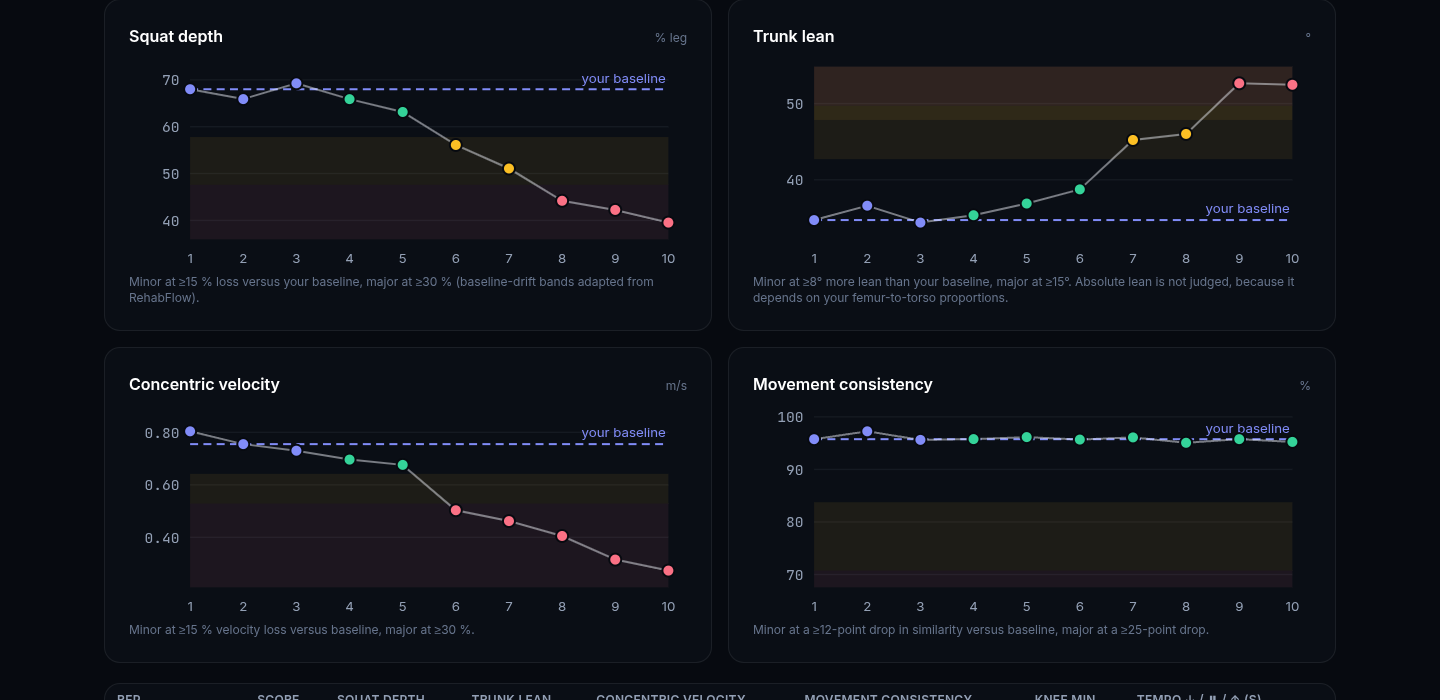
\includegraphics[width=0.8\textwidth]{rep-by-rep.png}
\caption{Per-metric drift charts for the simulated side-camera set. The dashed line is the baseline; the shaded areas are the minor and major bands.}
\end{figure}

\subsection{Repetition score and drift onset}

Each repetition starts at 100 points and loses up to each metric's weight in proportion to how far its deviation goes towards the major threshold:
\begin{equation}
\text{score} = 100 - \sum_{m} w_m \cdot \min\!\left(1.2,\ \frac{\max(0, \mathrm{dev}_m)}{\mathrm{major}_m}\right)
\end{equation}
The weights are 30 for depth, 30 for knee tracking, 25 for trunk lean, 20 for hip shift, 15 for velocity and 10 for consistency, so that safety and technique outweigh fatigue and consistency. A least-squares trend line, reported with its $R^2$, summarises how the score changes across the set.

\textbf{Drift onset} is the first repetition after the baseline that is flagged on a technique or safety metric together with the following repetition. Requiring two consecutive flagged repetitions suppresses one-off noise.

\begin{figure}[!htbp]
\centering
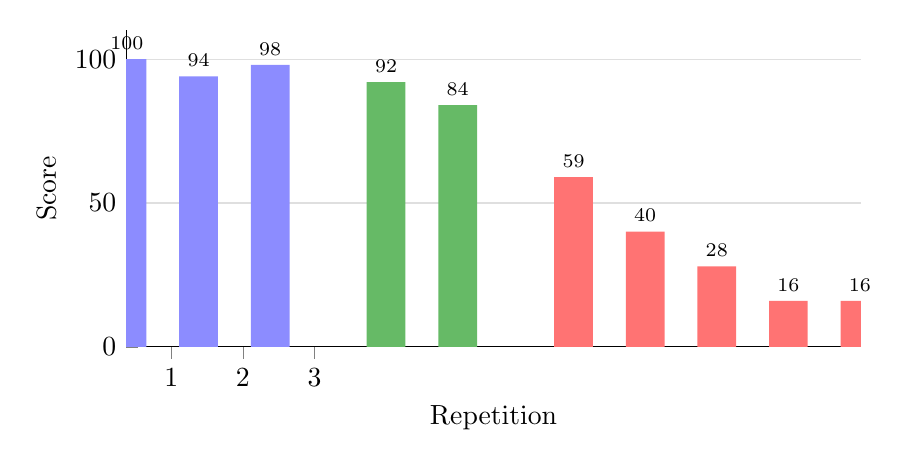
\begin{tikzpicture}
\begin{axis}[
    width=0.9\textwidth, height=5.6cm,
    ybar, bar width=14pt,
    ymin=0, ymax=110,
    xtick=data, xlabel={Repetition}, ylabel={Score},
    nodes near coords, nodes near coords style={font=\scriptsize},
    enlarge x limits=0.07,
    axis lines*=left, ymajorgrids, grid style={gray!25},
]
\addplot[fill=blue!45, draw=none] coordinates {(1,100) (2,94) (3,98)};
\addplot[fill=green!55!black!60, draw=none] coordinates {(4,92) (5,84)};
\addplot[fill=red!55, draw=none] coordinates {(6,59) (7,40) (8,28) (9,16) (10,16)};
\end{axis}
\end{tikzpicture}
\caption{Repetition scores for the simulated side-camera set. Repetitions 1--3 form the baseline (blue), 4--5 stay within the baseline (green), and drift is flagged from repetition 6 (red). The trend is $-11$ points per repetition with $R^2 = 0.92$.}
\end{figure}

\subsection{Lumbar load: a static L5/S1 model}

Forward trunk lean increases the load on the lower back. Following the static sagittal approach of Chaffin, Andersson and Martin (1999), the upper body is taken as 55\% of body mass with its centre of mass 40\% of the way up the trunk (de Leva, 1996). A load held at the chest is placed 75\% of the way up the trunk and 10 cm forward, and the erector spinae moment arm is 5 cm. With trunk length $L_t$ and trunk inclination $\theta$:
\begin{equation}
M = m_{ub}\, g\, (0.40\,L_t \sin\theta) + m_{load}\, g\, (0.75\,L_t \sin\theta + 0.10\cos\theta)
\end{equation}
\begin{equation}
F_c = \frac{M}{0.05} + (m_{ub} + m_{load})\, g \cos\theta
\end{equation}

For the real kettlebell clip (a 70 kg lifter with a 16 kg kettlebell) the estimate ranges from 1.46 to 1.61 kN, with the peak on the repetition with the most lean. The values are shown against the NIOSH action limit of 3.4 kN (Waters et al., 1993). The model is used only to compare repetitions within a set; it expresses the cost of extra lean in physical units (for example, ``8\% more spinal compression'') and makes no clinical claim.

\subsection{Signal processing}

Frames are sampled at 15 frames per second by seeking through the video, so results are deterministic and do not depend on playback speed. The pipeline then fills gaps of up to 0.6 s by linear interpolation, smooths the signals with a zero-phase Gaussian filter, and segments repetitions on the depth signal with a threshold of 0.35 times the peak. Dips shorter than 0.3 s are merged, hip hinges (minimum knee angle above 140\degree) and incomplete repetitions are rejected, and the descent and ascent are timed from the 15\% and 90\% depth crossings with sub-frame interpolation.

\begin{figure}[!htbp]
\centering
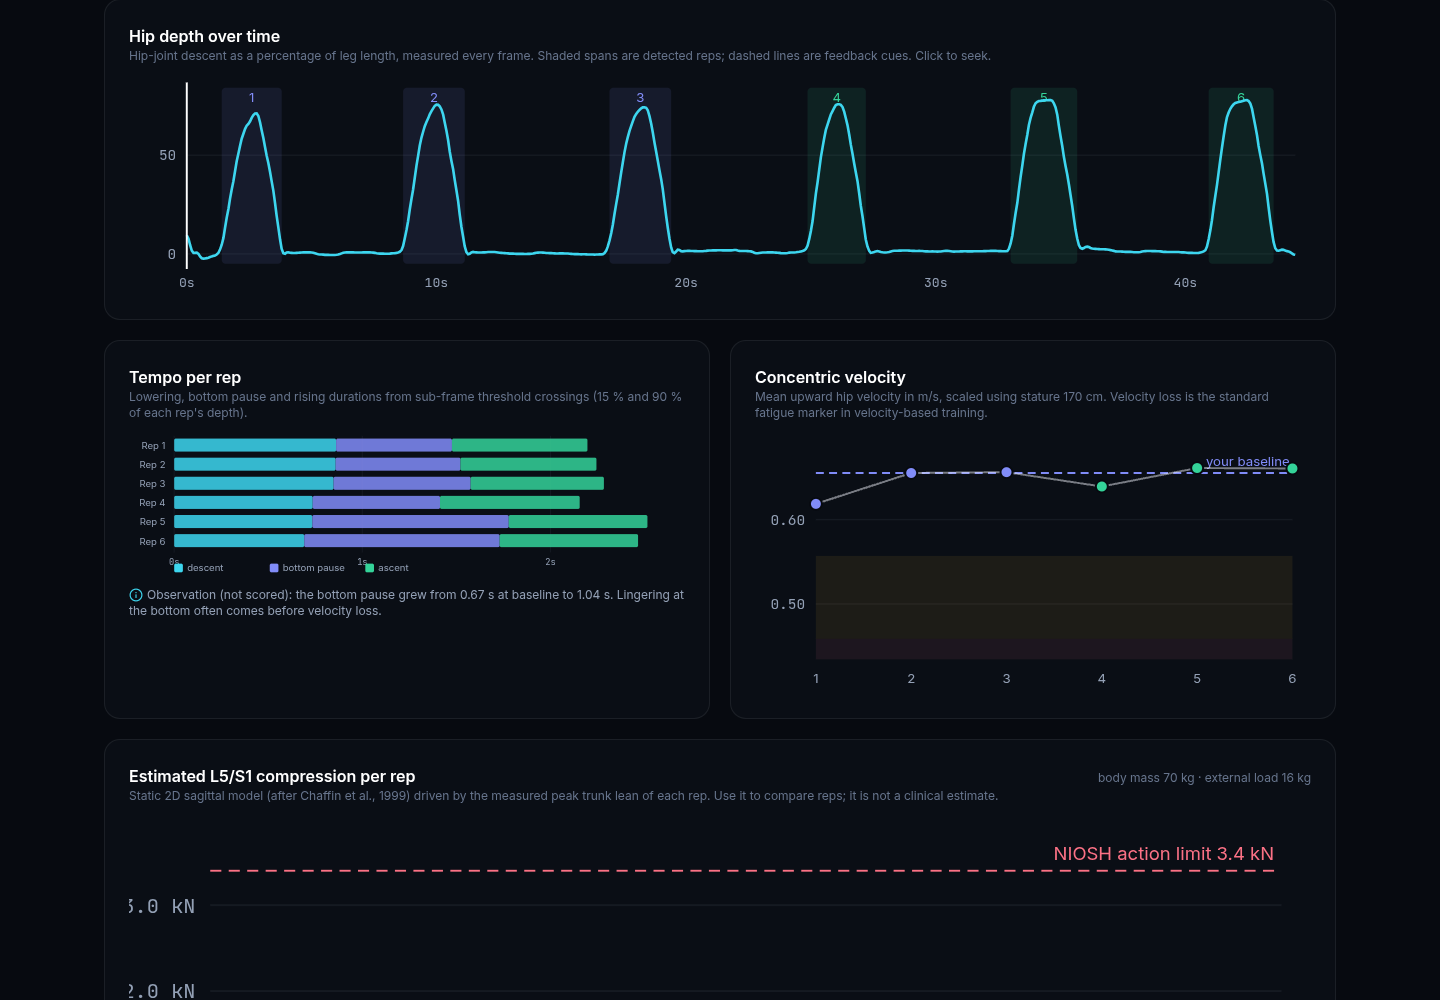
\includegraphics[width=0.64\textwidth]{biomechanics.png}
\caption{Biomechanics tab for the real kettlebell squat: estimated L5/S1 compression per repetition against the NIOSH action limit, and the tempo of each repetition.}
\end{figure}

%=====================================================================
\section{Information Handling}

\subsection{Constraints on feedback during a set}

During a set the lifter is under physical load, often cannot see the screen, and has little spare attention. Feedback that adds workload can harm the movement it is meant to improve. Every rule of the cue engine follows from these constraints (Table~\ref{tab:cues}).

\begin{table}[!htbp]
\centering
\caption{Cue rules, their implementation and their basis in the literature.}
\label{tab:cues}
\small
\begin{tabularx}{\textwidth}{>{\raggedright\arraybackslash}p{2.8cm} >{\raggedright\arraybackslash}p{5.4cm} L}
\toprule
\textbf{Rule} & \textbf{Implementation} & \textbf{Basis} \\
\midrule
One cue per repetition, at the right moment & Given when the repetition ends (standing), never at the bottom & Avoids interrupting the most demanding phase; terminal feedback suits motor learning (Sigrist et al., 2013). \\
Few words, external focus & ``Sit deeper'', ``Chest up'', ``Knees out'', ``Even weight'', ``Consider stopping'' & External-focus instructions improve performance and learning (Wulf, 2013); two words fit working memory under load. \\
Priority & Safety, then major technique, then minor technique, then fatigue, then consistency & The most important problem is addressed first. \\
Throttling & 3 s cooldown; the same cue at most twice in a row (three times if major) & Prevents nagging and habituation (Sigrist et al., 2013). \\
Escalate once & When two or more metrics are major for two repetitions in a row: ``End the set'', then silence & Further corrections stop helping once technique has broken down. \\
Choice of channel & Combined, visual only, audio only, haptic only or silent & Audio leaves the visual channel free (Wickens, 2002); haptic suits noisy gyms; silent defers everything to the summary. \\
Glanceable visual & A large ring (purple while calibrating, then green, amber or red) with a text label; no numbers on the athlete view & Readable from 3 m; colour is never the only code. \\
Details after the set & Charts, numbers, explanations and drills appear only in the summary & Separates the load during the set from reflective analysis afterwards. \\
\bottomrule
\end{tabularx}
\end{table}

\subsection{Cue engine behaviour}

The Feedback log lists every candidate cue, including the ones that were held back and the reason (``cooldown'', ``repeat limit'' or ``stop already recommended''), so the rules can be inspected. In the simulated side-camera set the engine produced ``Baseline set'' after repetition 3, ``Sit deeper'' at repetition 6, ``Chest up'' at 7, ``Sit deeper'' at 8 and ``End the set'' at 9, and suppressed a further cue at repetition 10.

\begin{figure}[!htbp]
\centering
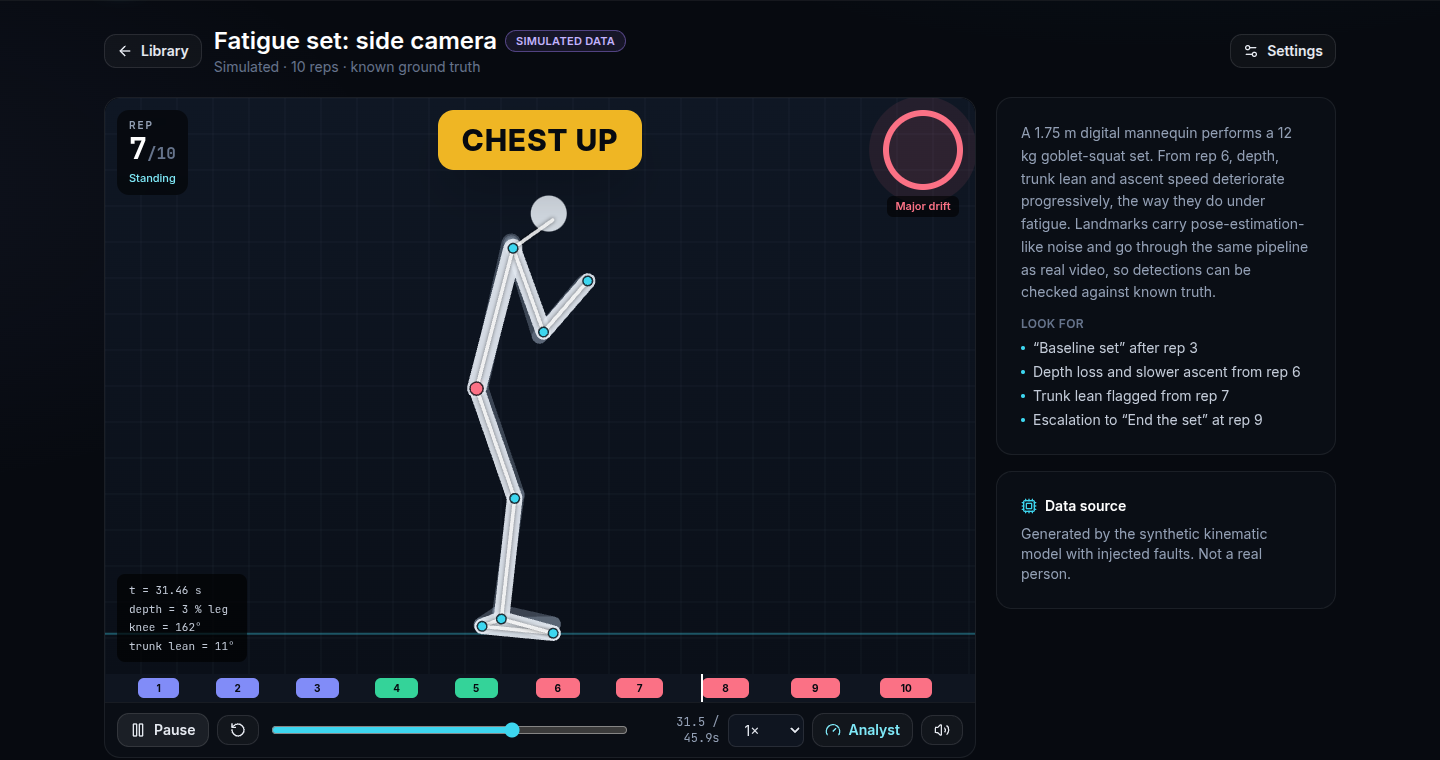
\includegraphics[width=0.64\textwidth]{player-cue.png}
\caption{The athlete view during playback: repetition counter (top left), a single cue (top centre), the status ring (top right) and the coloured repetition timeline.}
\end{figure}

%=====================================================================
\section{Aesthetic Evaluation and Interface Design}

Affective needs such as trust, comfort and motivation are served by the ``art'' of the interface.

\textbf{Legibility.} The interface uses a dark, high-contrast palette with one accent colour, generous spacing and tabular numerals. Three status colours (green, amber and red) are always paired with a text label so that colour-blind users are not excluded.

\textbf{Source labelling.} Every result carries a badge: \emph{Real video, measured}; \emph{Simulated data}; or \emph{Your video, measured}. Metrics that the camera view cannot support are listed as ``not measurable from this view'', and the synthetic figure is clearly drawn as a mannequin. A system that tells people their form is wrong needs to be trusted, and that trust should match what the system can actually measure.

\textbf{Self-perception check.} Before the results appear, the user is asked ``When did your form start to slip?''. The answer is compared with the measured onset, for example ``You noticed 2 reps later than the measured onset''. This turns the human issue into a personal observation that the user remembers.

\textbf{Framing.} Results explain what changed, why it matters and what to do (a corrective drill), instead of only scoring the person.

\textbf{Instruments.} The Study page provides the System Usability Scale (Brooke, 1996) and the raw NASA Task Load Index (Hart and Staveland, 1988), stored on the device with CSV export.

\begin{figure}[!htbp]
\centering
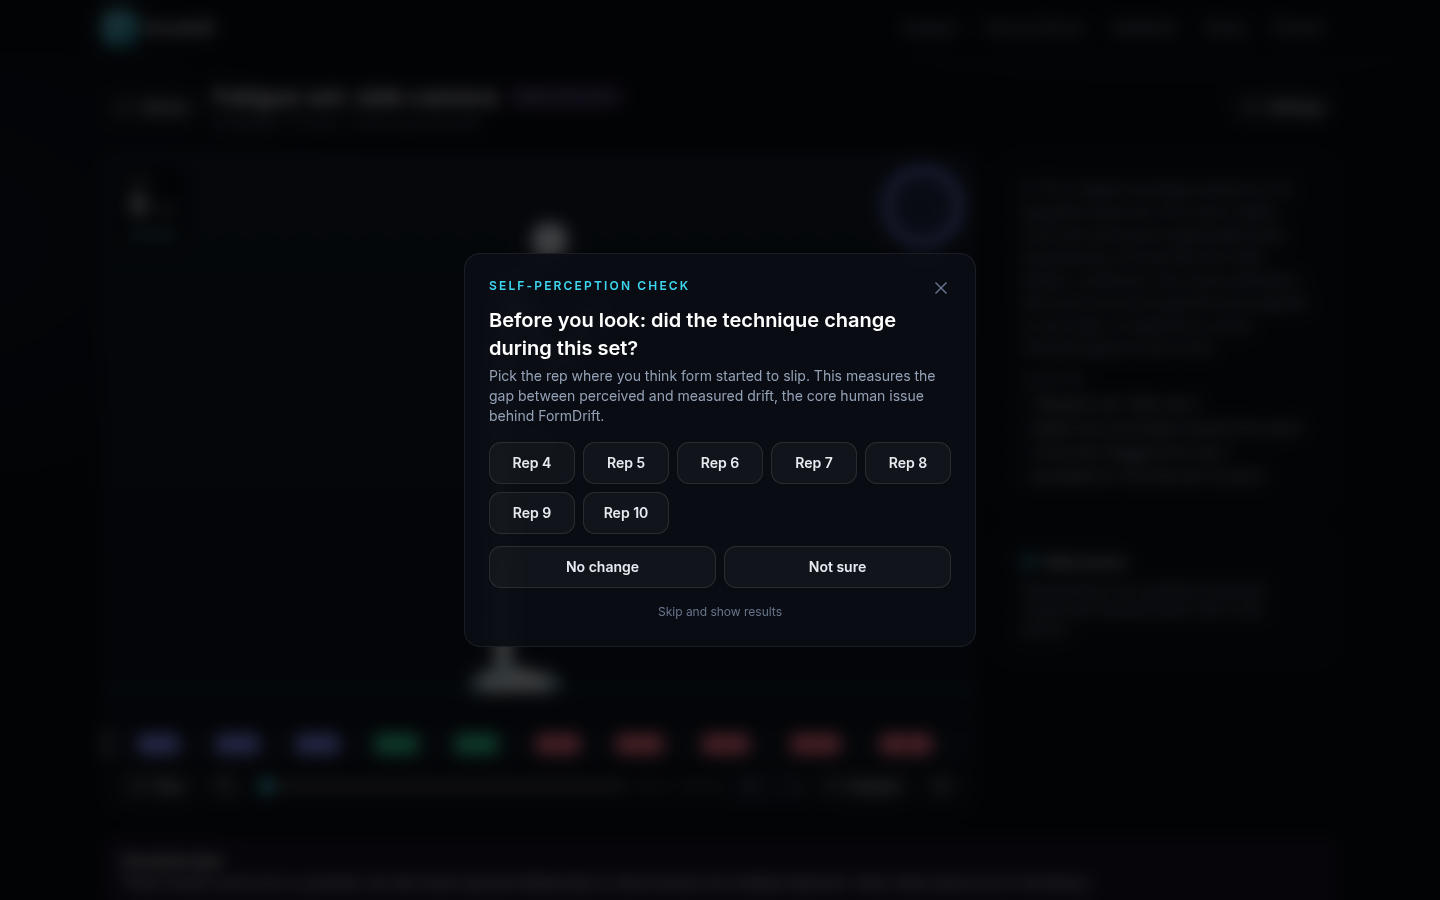
\includegraphics[width=0.6\textwidth]{perception-check.png}
\caption{Self-perception check, shown before any results.}
\end{figure}

\begin{figure}[!htbp]
\centering
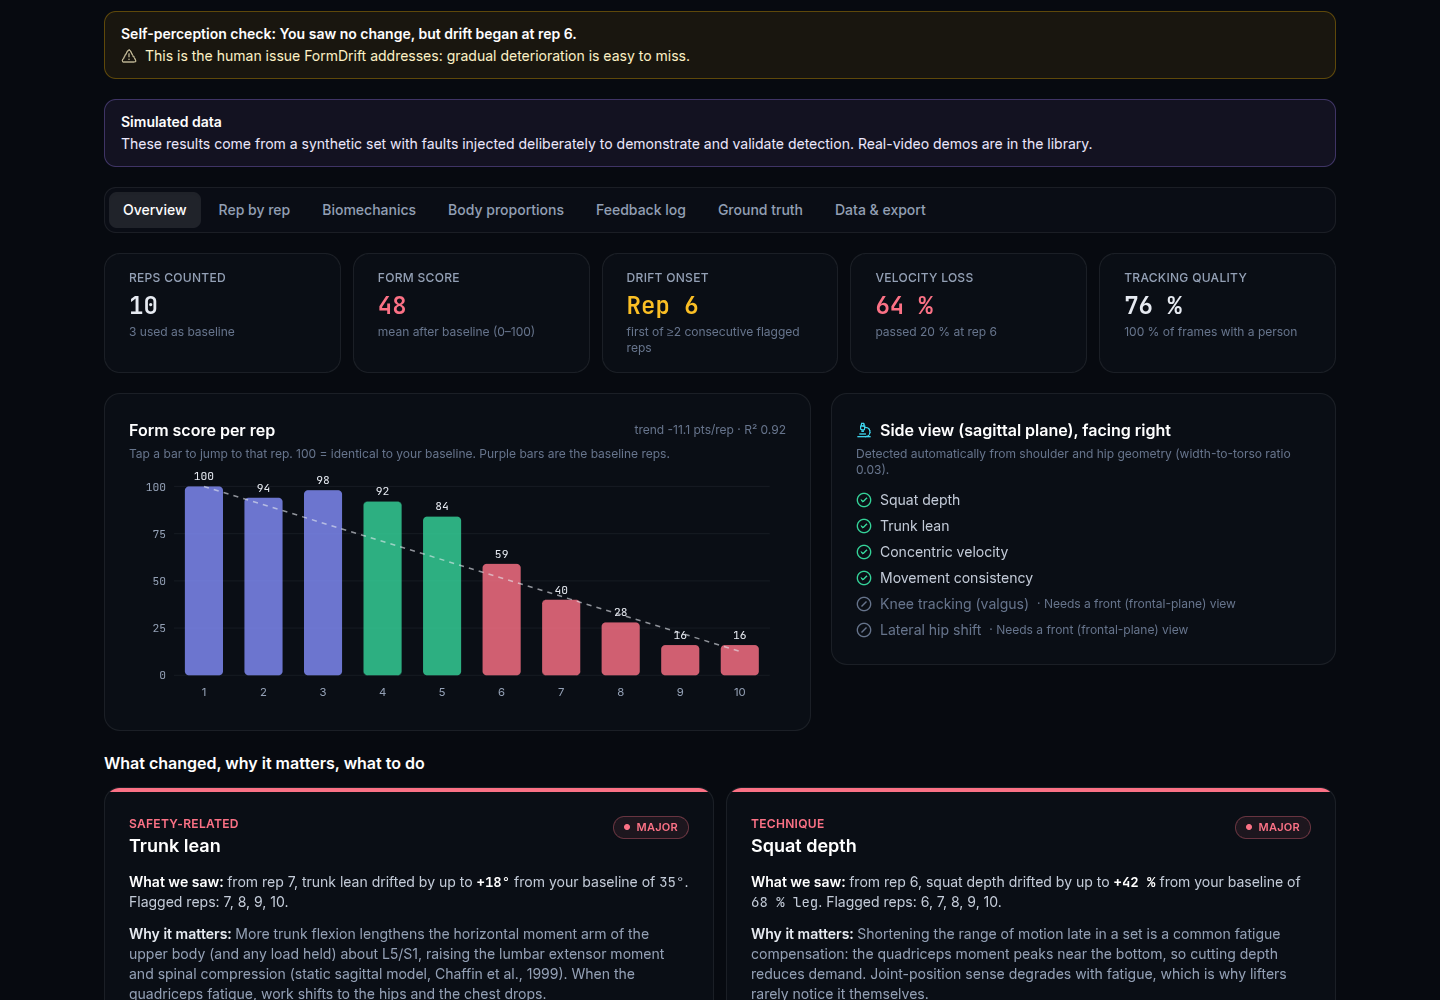
\includegraphics[width=0.6\textwidth]{overview.png}
\caption{Overview of the results for the simulated side-camera set: summary statistics, the score per repetition, the metrics available from this view and the explanation cards.}
\end{figure}

%=====================================================================
\section{Implementation}

\subsection{Architecture}

FormDrift is a static Progressive Web App with no backend. The processing pipeline is:

\begin{enumerate}
    \item \textbf{Pose estimation.} MediaPipe Pose Landmarker (WebAssembly and WebGL) returns 33 image landmarks and 33 world landmarks per frame, sampled at 15 frames per second.
    \item \textbf{Signal processing.} Gap filling, zero-phase Gaussian smoothing and leg-length normalisation.
    \item \textbf{View classification.} Side, front or oblique, from the shoulder and hip width relative to torso length.
    \item \textbf{Repetition segmentation.} Hysteresis on depth, rejection of hinges and incomplete repetitions, sub-frame tempo.
    \item \textbf{Per-repetition metrics and baseline.} Deviation from the median of the first $N$ repetitions, classified as ok, minor or major.
    \item \textbf{Outputs.} Score, trend, drift onset and issues feed the cue engine, the player overlay and the post-set summary.
\end{enumerate}

\begin{table}[!htbp]
\centering
\caption{Technology choices.}
\small
\begin{tabularx}{\textwidth}{>{\raggedright\arraybackslash}p{3.0cm} >{\raggedright\arraybackslash}p{5.6cm} L}
\toprule
\textbf{Concern} & \textbf{Choice} & \textbf{Reason} \\
\midrule
Pose estimation & MediaPipe Tasks Vision, Pose Landmarker (full model), GPU with CPU fallback & Mature, Apache-2.0 licensed, runs in the browser, provides 3D world landmarks \\
Front end & Vite, React 19, TypeScript, Tailwind CSS 4 & Fast to build, typed and maintainable \\
PWA & vite-plugin-pwa (Workbox) & Precaches the app, demo clips and landmark data; caches the model and WebAssembly at run time \\
Routing & Hash routing with a relative base path & Works on any static host or sub-path \\
Charts & Hand-written SVG & No extra dependency, sharp at any size \\
Feedback output & Web Speech API, Vibration API, canvas overlay & Built into browsers; no hardware needed \\
Storage & Browser local storage & Profile and study responses stay on the device \\
\bottomrule
\end{tabularx}
\end{table}

\begin{figure}[!htbp]
\centering
\begin{subfigure}[b]{0.72\textwidth}
\centering
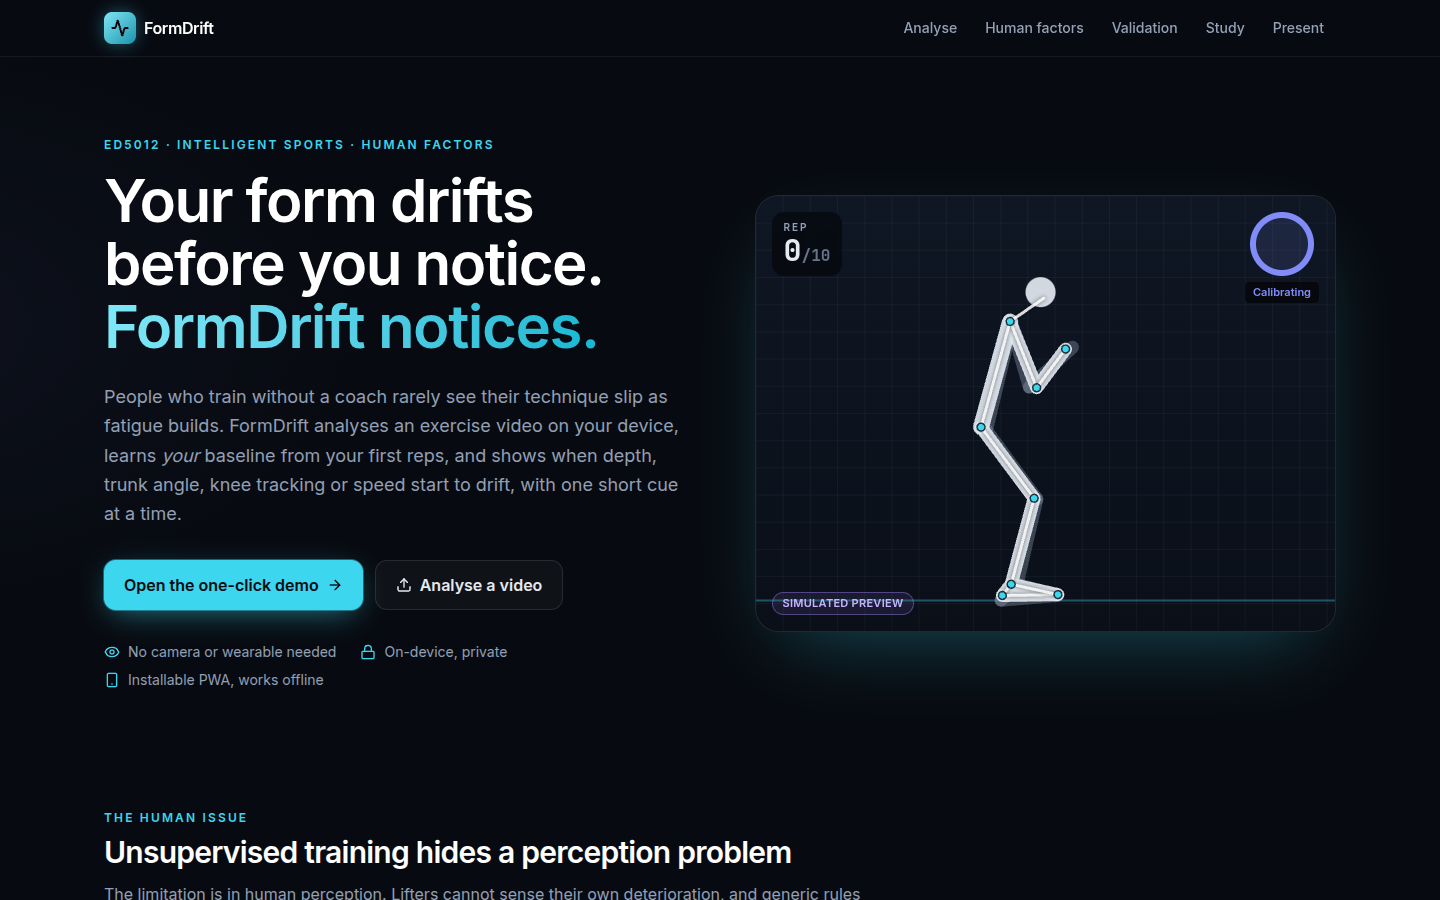
\includegraphics[width=\textwidth]{landing.png}
\caption{Landing page on a laptop.}
\end{subfigure}\hfill
\begin{subfigure}[b]{0.24\textwidth}
\centering
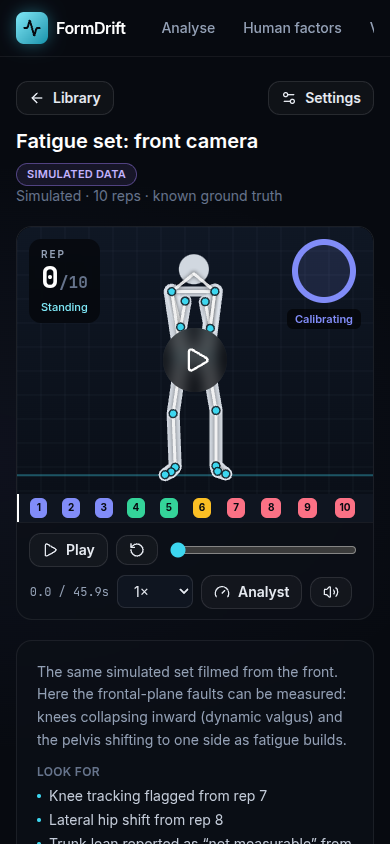
\includegraphics[width=\textwidth]{mobile-session.png}
\caption{Session view on a phone.}
\end{subfigure}
\caption{The same PWA serves a laptop for review and a phone in the gym.}
\end{figure}

\subsection{Demo mode}

The demonstration had to work reliably on a laptop over Google Meet, without a camera or any hardware, and without overstating what the analysis can do. FormDrift therefore offers four preloaded sets (Table~\ref{tab:demo}). Users can also upload their own video, which is processed in the browser.

\begin{table}[!htbp]
\centering
\caption{Preloaded demonstration sets.}
\label{tab:demo}
\small
\begin{tabularx}{\textwidth}{>{\raggedright\arraybackslash}p{4.2cm} >{\raggedright\arraybackslash}p{4.6cm} L}
\toprule
\textbf{Set} & \textbf{Source} & \textbf{Purpose} \\
\midrule
Fatigue set, side camera & Synthetic kinematic model, 10 repetitions & Depth loss, trunk lean and velocity loss, with ground truth \\
Fatigue set, front camera & Same model, frontal projection & Knee valgus and hip shift, with ground truth \\
Kettlebell squat, side view & Real video (CC BY-SA 4.0) & Real MediaPipe measurement; checks that consistent lifting raises no alarms \\
Barbell back squat, oblique & Real video (CC BY-SA 4.0) & Shows how an oblique camera is handled \\
\bottomrule
\end{tabularx}
\end{table}

The landmarks of the real clips were extracted with the app's own in-browser pipeline and stored, so the demonstration opens instantly. A \emph{Re-extract live with MediaPipe} button runs the extraction again in the browser; in testing, live extraction reproduced the stored results exactly.

\subsection{Synthetic fatigue model}

The synthetic model is a 3D stick figure with Drillis and Contini segment lengths for a stature of 1.75 m. It performs goblet squats with a 1.6 s descent, a 0.3 s pause and a 1.25 s ascent. A fatigue pattern is introduced gradually from repetition 4 and becomes large from repetition 6: depth falls to 72\% of the original, trunk lean rises by up to 27\degree, the ascent slows by up to 62\%, knee valgus reaches 5.6 cm and hip shift reaches 5.8 cm. The model is projected onto a $640 \times 480$ camera with 2.2-pixel Gaussian noise and reduced visibility on the far side, which resembles MediaPipe output. Ground truth is taken from the noise-free 3D model.

\subsection{Reuse of existing work and licensing}

\begin{table}[!htbp]
\centering
\caption{External work used and its licence.}
\small
\begin{tabularx}{\textwidth}{>{\raggedright\arraybackslash}p{4.6cm} >{\raggedright\arraybackslash}p{2.6cm} L}
\toprule
\textbf{Source} & \textbf{Licence} & \textbf{Use} \\
\midrule
MediaPipe Tasks Vision and the Pose Landmarker model (Google) & Apache-2.0 & Dependency, self-hosted for offline use \\
TechnIQ form coach (younis-y) & MIT & Ideas adapted (per-repetition scoring, trend with $R^2$, fault and drill presentation) and rewritten in TypeScript \\
RehabFlow, wwm, FormGuard & No licence & No code used; general ideas reimplemented independently \\
Fitness-AQA (Parmar and Morris, 2022) & Research use & Supports the fault taxonomy only \\
Demo videos (Taco Fleur; Your Move) via Wikimedia Commons & CC BY-SA 4.0 & Trimmed, cropped and re-encoded, with attribution in the app \\
\bottomrule
\end{tabularx}
\end{table}

\subsection{Quality assurance and deployment}

Fourteen automated regression checks (\texttt{npm run verify}) cover repetition counts, view classification, an F1 score of at least 0.95, drift onset and the absence of false alarms on the real clips; they run on every push through GitHub Actions. A headless browser test (\texttt{npm run smoke}) visits every page and tab of every demo set, the slides and a phone-sized viewport, and fails on any console error. An error boundary prevents a failure on one page from blanking the whole app.

The production build is a set of static files. It is published at \url{https://formdrift.apps.grok.bot}, and the repository also contains a GitHub Pages workflow that can serve the same build from the repository as a second copy. Once loaded, the app is cached by its service worker and keeps working without a network connection, including the demo videos.


%=====================================================================
\section{Functional Evaluation}

Functional evaluation asks whether the system does what it claims. FormDrift was evaluated at three levels, all of which are computed live on the Validation page of the app: measurement against known truth, specificity on real video, and robustness to landmark noise.

\subsection{Simulation with known ground truth}

The analysis was run on the simulated sets, and the level (ok, minor or major) assigned to each repetition after the baseline was compared with the level that the true values deserve under the same baseline rule.

\begin{table}[!htbp]
\centering
\caption{Measurement error and drift-flag confusion counts on the simulated sets (TP: true positive, FP: false positive, FN: false negative, TN: true negative).}
\small
\begin{tabular}{l c l r c c c c c}
\toprule
\textbf{Camera} & \textbf{Reps} & \textbf{Metric} & \textbf{MAE} & \textbf{TP} & \textbf{FP} & \textbf{FN} & \textbf{TN} & \textbf{Agreement} \\
\midrule
\multirow{3}{*}{Side} & \multirow{3}{*}{10/10} & Squat depth & 0.69\% leg & 5 & 0 & 0 & 2 & 100\% \\
 & & Trunk lean & 0.77\degree & 4 & 0 & 0 & 3 & 100\% \\
 & & Concentric velocity & 0.027 m/s & 5 & 0 & 0 & 2 & 86\% \\
\midrule
\multirow{4}{*}{Front} & \multirow{4}{*}{10/10} & Squat depth & 0.25\% leg & 5 & 0 & 0 & 2 & 100\% \\
 & & Knee tracking & 1.39\% & 4 & 0 & 0 & 3 & 100\% \\
 & & Lateral hip shift & 0.84\% & 3 & 0 & 0 & 4 & 100\% \\
 & & Concentric velocity & 0.016 m/s & 5 & 0 & 0 & 2 & 100\% \\
\bottomrule
\end{tabular}
\end{table}

Overall drift-flag precision and recall were both 1.00 for both cameras. In both sets drift onset was detected at repetition 6, and velocity loss passed 20\% at repetition 6. Mean scores fell from about 97--99 in the baseline repetitions to 48 (side) and 39 (front) after the baseline, with trends of $-11$ and $-13$ points per repetition ($R^2 = 0.92$). The single level disagreement (side camera, velocity, one repetition) is a boundary case between minor and major; no drift was missed.

\subsection{Real video: repetition counting and specificity}

\begin{table}[!htbp]
\centering
\caption{Results on the two real clips.}
\small
\begin{tabularx}{\textwidth}{L >{\raggedright\arraybackslash}p{2.6cm} c c c c c}
\toprule
\textbf{Clip} & \textbf{View detected} & \textbf{Manual} & \textbf{Detected} & \textbf{Alarms} & \textbf{Score} & \textbf{Pose found} \\
\midrule
Kettlebell squat, side, backlit outdoors & Side (ratio 0.04) & 6 & 6 & 0 & 97 & 100\% \\
Barbell back squat, studio & Oblique (ratio 0.32) & 4 & 4 & 0 & 98 & 100\% \\
\bottomrule
\end{tabularx}
\end{table}

Both clips show an experienced lifter with consistent technique, so the correct behaviour is to count every repetition and raise no alarm, and FormDrift did so. It still reported the real variation it measured as information. In the kettlebell set the bottom pause grew from 0.62 s to 1.04 s in repetitions 5 and 6, and peak L5/S1 compression rose by about 8\%. In the barbell set velocity fell by 10\% on the last repetition, which is below the threshold. For the oblique clip, trunk lean and knee valgus were reported as not measurable.

\begin{figure}[!htbp]
\centering
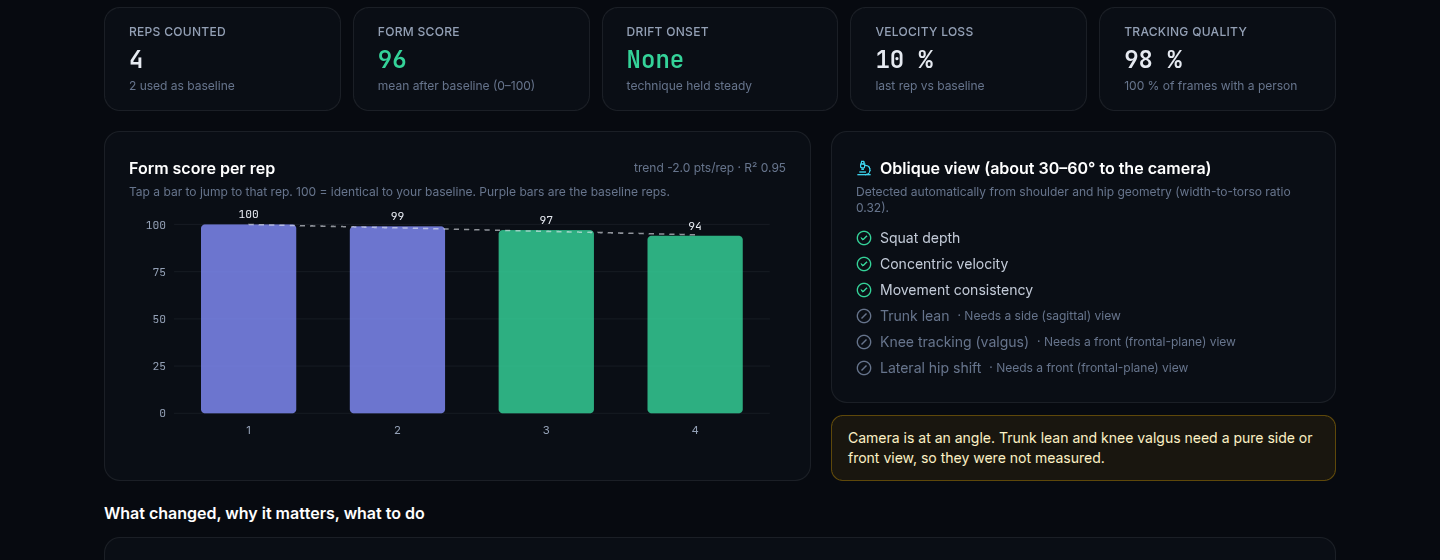
\includegraphics[width=0.9\textwidth]{oblique-view.png}
\caption{Oblique barbell clip: repetitions are counted, and metrics that this view cannot support are marked as not measurable.}
\end{figure}

\subsection{Robustness to landmark noise}

Gaussian noise of 0 to 10 pixels was added to the simulated landmarks in a $640 \times 480$ frame, with three random seeds per noise level.

\begin{figure}[!htbp]
\centering
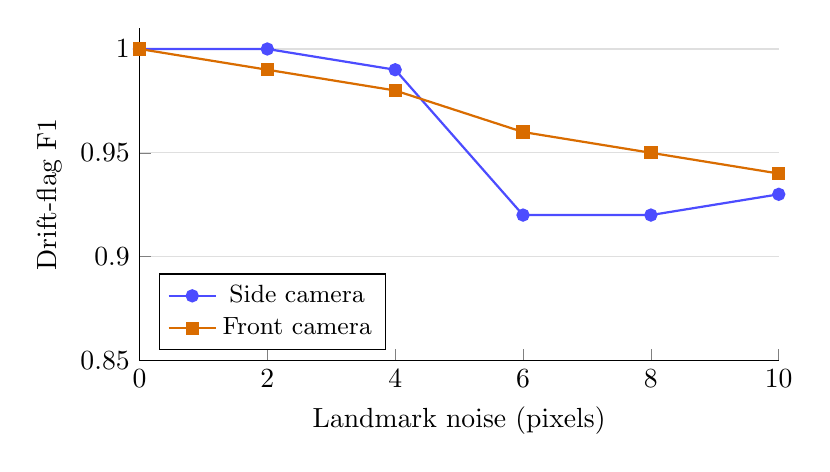
\begin{tikzpicture}
\begin{axis}[
    width=0.8\textwidth, height=5.8cm,
    xlabel={Landmark noise (pixels)}, ylabel={Drift-flag F1},
    xmin=0, xmax=10, ymin=0.85, ymax=1.01,
    xtick={0,2,4,6,8,10},
    legend pos=south west, legend style={font=\small},
    ymajorgrids, grid style={gray!25}, axis lines*=left,
]
\addplot[mark=*, thick, color=blue!70] coordinates {(0,1.00) (2,1.00) (4,0.99) (6,0.92) (8,0.92) (10,0.93)};
\addlegendentry{Side camera}
\addplot[mark=square*, thick, color=orange!85!black] coordinates {(0,1.00) (2,0.99) (4,0.98) (6,0.96) (8,0.95) (10,0.94)};
\addlegendentry{Front camera}
\end{axis}
\end{tikzpicture}
\caption{Drift-flag F1 against landmark noise (mean of three seeds). The repetition count was exact at every noise level.}
\end{figure}

Typical MediaPipe jitter on good video is about 2 to 4 pixels, where F1 is 0.98 or higher. Performance degrades gradually, and precision stays at or above 0.93, so noise leads to occasional missed minor flags rather than false alarms. For user trust, this is the safer way to fail.

\subsection{Self-protection against unreliable input}

Each repetition receives a confidence score (landmark visibility multiplied by detection rate). Repetitions below 0.45 are marked as low confidence and are never flagged. Quality warnings appear when the person is detected in fewer than 85\% of frames or the feet are out of frame, and an oblique-view warning explains which metrics were not measured.

%=====================================================================
\section{Planned User Study}

A formal study with participants was outside the scope of the course, so no participant data is reported here. The Study page of the app implements a protocol that is ready to run.

\begin{itemize}
    \item \textbf{Participants:} 8 to 12 recreational lifters with at least six months of training, varied in stature and sex, with informed consent.
    \item \textbf{Design:} within-subjects and counterbalanced, with three conditions: no feedback, audio cues and visual cues only. Each condition is one set of 10 to 12 goblet or back squats taken close to failure, filmed side-on at hip height from 2 to 3 m.
    \item \textbf{Measures:} drift onset, flagged repetitions, depth and lean deviation and velocity loss; perceived onset from the self-perception check, giving an awareness gap (perceived minus measured onset); SUS, raw NASA-TLX and preferred modality.
    \item \textbf{Hypotheses:} H1, without feedback, perceived onset comes later than measured onset; H2, sets with cues contain fewer repetitions with major drift; H3, SUS is at least 68 and workload is lower for audio cues than for visual cues.
    \item \textbf{Analysis:} Wilcoxon signed-rank tests with effect sizes, appropriate for a small sample.
\end{itemize}

%=====================================================================
\section{Limitations}

\begin{enumerate}
    \item \textbf{A single 2D camera.} Out-of-plane motion is foreshortened. Metrics are restricted by view to limit this, but a side camera cannot see valgus and a front camera cannot see trunk lean.
    \item \textbf{Thresholds} come from the literature and from the 15\%/30\% convention used in rehabilitation tools. They have not been calibrated against expert ratings.
    \item \textbf{The simulation validates the measurement and decision pipeline}, not the realism of the fatigue pattern, which varies between people.
    \item \textbf{The real clips show consistent technique.} They demonstrate that the system does not raise false alarms, but not its sensitivity to real fatigue; that requires the user study.
    \item \textbf{Squat only, analysed after the set.} The cue engine is designed for live use, but a live camera mode was left out to keep the demonstration reliable and hardware-free.
    \item \textbf{The L5/S1 estimate} is a simplified static model for comparing repetitions, not an absolute or clinical measure.
    \item \textbf{MediaPipe accuracy} drops with loose clothing, occlusion by equipment, backlighting and low resolution. The app reports tracking quality and per-repetition confidence instead of hiding this.
    \item \textbf{Stature is entered by the user.} Velocity in metres per second is only as accurate as that input; relative velocity loss is unaffected.
\end{enumerate}

%=====================================================================
\section{Future Work}

\begin{itemize}
    \item Run the built-in study and report the awareness gap and the effect of feedback modality.
    \item Add a live camera mode using the same cue engine, and measure latency on mid-range phones.
    \item Extend the analysis to the deadlift (hinge segmentation) and the lunge, and add left-right asymmetry from a front view.
    \item Calibrate thresholds against coach ratings such as the Fitness-AQA labels, and personalise thresholds using the variability of the baseline repetitions.
    \item Optionally fuse the phone's motion sensors, attached to the bar, with video for velocity.
\end{itemize}

%=====================================================================
\section{Conclusion}

FormDrift addresses a human problem: people cannot perceive their own technique drifting as they tire. The solution is built around human capabilities at each level of the course framework: a personal baseline for anthropometry, view-dependent kinematics and a lumbar load model for biomechanics, one well-timed cue of a few words in a chosen modality for information handling, measured accuracy with stated limits for functional evaluation, and a legible, clearly labelled interface with a self-perception check for aesthetic evaluation. It runs entirely in a browser as an installable, offline PWA, so it can be demonstrated live without any hardware.

%=====================================================================
\section*{References}
\addcontentsline{toc}{section}{References}
\footnotesize
\begin{enumerate}
\setlength{\itemsep}{2pt}
\item Bazarevsky, V., Grishchenko, I., Raveendran, K., Zhu, T., Zhang, F., and Grundmann, M. (2020). BlazePose: On-device real-time body pose tracking. \emph{CVPR Workshop on Computer Vision for Augmented and Virtual Reality.}
\item Brooke, J. (1996). SUS: A ``quick and dirty'' usability scale. In P. W. Jordan et al. (Eds.), \emph{Usability Evaluation in Industry} (pp. 189--194). Taylor and Francis.
\item Chaffin, D. B., Andersson, G. B. J., and Martin, B. J. (1999). \emph{Occupational Biomechanics} (3rd ed.). Wiley.
\item Chakrabarti, D. (1997). \emph{Indian Anthropometric Dimensions for Ergonomic Design Practice.} National Institute of Design, Ahmedabad.
\item de Leva, P. (1996). Adjustments to Zatsiorsky-Seluyanov's segment inertia parameters. \emph{Journal of Biomechanics, 29}(9), 1223--1230.
\item Gonz\'alez-Badillo, J. J., and S\'anchez-Medina, L. (2010). Movement velocity as a measure of loading intensity in resistance training. \emph{International Journal of Sports Medicine, 31}(5), 347--352.
\item Hart, S. G., and Staveland, L. E. (1988). Development of NASA-TLX (Task Load Index): Results of empirical and theoretical research. \emph{Advances in Psychology, 52}, 139--183.
\item Myer, G. D., Kushner, A. M., Brent, J. L., et al. (2014). The back squat: A proposed assessment of functional deficits and technical factors that limit performance. \emph{Strength and Conditioning Journal, 36}(6), 4--27.
\item Noyes, F. R., Barber-Westin, S. D., Fleckenstein, C., Walsh, C., and West, J. (2005). The drop-jump screening test: Difference in lower limb control by gender and effect of neuromuscular training in female athletes. \emph{American Journal of Sports Medicine, 33}(2), 197--207.
\item Pareja-Blanco, F., Rodr\'iguez-Rosell, D., S\'anchez-Medina, L., et al. (2017). Effects of velocity loss during resistance training on athletic performance, strength gains and muscle adaptations. \emph{Scandinavian Journal of Medicine and Science in Sports, 27}(7), 724--735.
\item Parmar, P., and Morris, B. (2022). Domain knowledge-informed self-supervised representations for workout form assessment. \emph{European Conference on Computer Vision (ECCV).}
\item Proske, U., and Gandevia, S. C. (2012). The proprioceptive senses: Their roles in signaling body shape, body position and movement, and muscle force. \emph{Physiological Reviews, 92}(4), 1651--1697.
\item Sanders, M. S., and McCormick, E. J. (1993). \emph{Human Factors in Engineering and Design} (7th ed.). McGraw-Hill.
\item Sigrist, R., Rauter, G., Riener, R., and Wolf, P. (2013). Augmented visual, auditory, haptic, and multimodal feedback in motor learning: A review. \emph{Psychonomic Bulletin and Review, 20}(1), 21--53.
\item Waters, T. R., Putz-Anderson, V., Garg, A., and Fine, L. J. (1993). Revised NIOSH equation for the design and evaluation of manual lifting tasks. \emph{Ergonomics, 36}(7), 749--776.
\item Wickens, C. D. (2002). Multiple resources and performance prediction. \emph{Theoretical Issues in Ergonomics Science, 3}(2), 159--177.
\item Winter, D. A. (2009). \emph{Biomechanics and Motor Control of Human Movement} (4th ed.). Wiley.
\item Wulf, G. (2013). Attentional focus and motor learning: A review of 15 years. \emph{International Review of Sport and Exercise Psychology, 6}(1), 77--104.
\end{enumerate}

\textbf{Software and media}
\begin{itemize}
\setlength{\itemsep}{2pt}
\item MediaPipe Tasks Vision, Google, Apache-2.0. \url{https://github.com/google-ai-edge/mediapipe}
\item TechnIQ form coach, younis-y, MIT. \url{https://github.com/younis-y/techniq-form-coach}
\item Fitness-AQA, Parmar and Morris. \url{https://github.com/ParitoshParmar/Fitness-AQA}
\item ``Kettlebell Racked Squats (side view)'', Taco Fleur, CC BY-SA 4.0, Wikimedia Commons.
\item ``Barbell back squat exercise demonstration'', Your Move (ymove.app), CC BY-SA 4.0, Wikimedia Commons.
\end{itemize}
\normalsize

%=====================================================================
\appendix
\section{Running the Application}
\small
\textbf{Online:} open \url{https://formdrift.apps.grok.bot} in a recent browser. After the first visit the app works offline and can be installed from the address bar. \textbf{Locally} (Node.js 20 or later): \texttt{git clone https://github.com/vinnay4/ED5012.git}, then \texttt{npm ci} and \texttt{npm run dev} (development server on port 5173), \texttt{npm run build} (static build in \texttt{dist/}) and \texttt{npm run verify} (14 regression checks).
\normalsize

\end{document}
